\subsection{UC4 - Impostazioni visualizzazione}
\label{uc4}

    \begin{figure}[htbp]
        \centering
        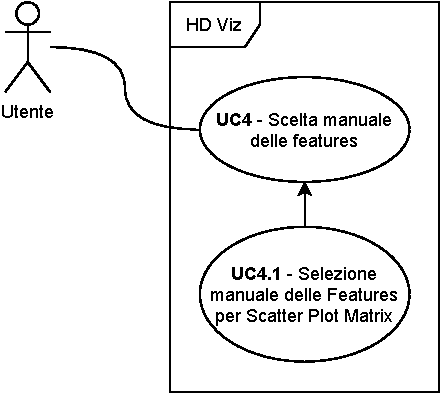
\includegraphics[width=0.7\textwidth]{source/sections/casi-uso/diagrams/uc4.pdf}
        \caption{UC4 - Impostazioni visualizzazione}
        \label{fig:uc4}
    \end{figure}

\begin{itemize}
    \item \textbf{Attore}: utente;
    \item \textbf{Descrizione}: l'utente, dopo che ha selezionato un tipo di visualizzazione tra Scatter Plot Matrix, Force Field, Linear Projection e Parallel Coordinates, modifica le impostazioni con cui visualizza il dato.
    \item \textbf{Precondizione}: 
    \begin{itemize}
        \item eseguito l'upload del dataset come matrice $N\times M$ (\hyperref[uc1]{UC1});
        \item selezionata una tra le visualizzazioni Scatter Plot Matrix (\hyperref[uc2.1.1]{UC2.1.1}), Force Field (\hyperref[uc2.1.4]{UC2.1.4}), Linear Projection (\hyperref[uc2.1.5]{UC2.1.5}), Parallel Coordinates.
    \end{itemize}  
    \item \textbf{Postcondizione}: l'utente ha regolato secondo le proprie necessità le impostazioni relative alla visualizzazione scelta;
    \item \textbf{Scenario Principale}: 
    \begin{enumerate}
        \item l'utente sceglie se e quale classe di visualizzazione assegnare a una variabile target; (\hyperref[uc4.1]{UC4.1});
    \end{enumerate}  
    \end{itemize}


 \subsubsection{UC4.1 - Assegnazione delle classi di visualizzazione alle variabili target}
    \label{uc4.1}
    \begin{itemize}
    \item \textbf{Attore}: utente;
    \item \textbf{Descrizione}: l'utente decide di assegnare dei diversi modi per distinguere un punto nel grafico, assegnando una classe di visualizzazione (colore, forma, size) ad ogni variabile target, in questo modo risulta più semplice per l'analista vedere dei pattern nella visualizzazione del grafico;
    \item \textbf{Precondizione}:
    \begin{itemize}
        \item eseguito l'upload del dataset come matrice $N\times M$ (\hyperref[uc2.1]{UC2.1});
        \item selezionato una tra le visualizzazioni Scatter Plot Matrix (\hyperref[uc2.1.1]{UC2.1.1}), Force Field (\hyperref[uc2.1.4]{UC2.1.4}) Linear Projection (\hyperref[uc2.1.5]{UC2.1.5});
        \item nel dataset, almeno una feature è stata selezionata come variabile target
    \end{itemize}
    \item \textbf{Postcondizione}: al variare del valore della variabile target $X$, i punti visualizzati assumono un diverso attributo della classe assegnata a quest'ultima;
    \item \textbf{Scenario Principale}: 
    \begin{enumerate}
        \item l'utente visualizza tutte le variabili target selezionate;
        \item l'utente associa ad ogni variabile target una classe di visualizzazione.
    \end{enumerate}  
    \end{itemize}
    
    \subsubsection{UC4.2 - Modificare il range}
    \label{uc4.2}
    \begin{itemize}
    \item \textbf{Attore}: utente;
    \item \textbf{Descrizione}: l'utente decide di modificare il range (range di $\textrm{default}=[min, max]$ dove $min=\textrm{valore minimo presente nel dataset}$ e $max=\textrm{valore massimo presente nel dataset}$), su cui ogni valore assume una diversa sfumatura di colore, cioè se viene scelto un range $[min, max-i]$, tutti i valori $\geq max-i$ presenti nel dataset verranno visualizzati con lo stesso colore;
    \item \textbf{Precondizione}: 
    \begin{itemize}
        \item eseguito l'upload del dataset come matrice $N\times M$ (\hyperref[uc1]{UC1});
        \item selezionato Heatmap come visualizzazione (\hyperref[uc2.1.2]{UC2.1.2}).
    \end{itemize}  
    \item \textbf{Postcondizione}: ricolorazione della Heatmap in base al range selezionato;
    \item \textbf{Scenario Principale}: 
    \begin{enumerate}
        \item l'utente modifica i valori di minimo e massimo su cui il sistema andrà a eseguire la sfumatura del colore.
    \end{enumerate}  
    \end{itemize}
    
     \subsubsection{UC4.3 - Assegnare colore al range}
    \label{uc4.3}
    
    \begin{itemize}
    \item \textbf{Attore}: utente;
    \item \textbf{Descrizione}: l'utente seleziona i colori con cui vuole evidenziare i valori di una Heatmap;
    \item \textbf{Precondizione}: 
    \begin{itemize}
        \item selezionato Heatmap o Correlation Heatmap come visualizzazione (\hyperref[uc2.1.2]{UC2.1.2} o \hyperref[uc2.1.3]{UC2.1.3});
    \end{itemize}  
    \item \textbf{Postcondizione}: la Heatmap conterrà nelle sue caselle le sfumature del colore selezionato;
    \item \textbf{Scenario Principale}: 
    \begin{enumerate}
        \item l'utente seleziona il colore con cui vuole visualizzare la Heatmap.
    \end{enumerate}  
    \end{itemize}

    \subsubsection{UC4.4 - Ordinamento delle righe di una Heatmap}
    \label{uc4.4}
    
    \begin{itemize}
    \item \textbf{Attore}: utente;
    \item \textbf{Descrizione}: l'utente seleziona in che modo organizzare la visualizzazione delle righe di una heatmap, scegliendo tra l'ordine alfabetico o raggruppamento in clusters;
    \item \textbf{Precondizione}: 
    \begin{itemize}
        \item eseguito l'upload del dataset come matrice $N\times M$ (\hyperref[uc1]{UC1});
        \item selezionato Heatmap come visualizzazione (\hyperref[uc2.1.2]{UC2.1.2}).
    \end{itemize}  
    \item \textbf{Postcondizione}: riordinazione della Heatmap in base all'ordinamento selezionato;
    \item \textbf{Scenario Principale}: 
    \begin{enumerate}
        \item l'utente sceglie quale ordinamento desidera effettuare.
    \end{enumerate}  
    \item \textbf{Generalizzazioni}: 
     \begin{enumerate}
            \item l'utente sceglie quale tipo di ordinamento:
                \begin{enumerate}
                    \item ordine Alfabetico (\hyperref[uc4.4.1]{UC4.4.1});
                    \item raggruppamento in Clusters (\hyperref[uc4.4.2]{UC4.4.2}).
                    \end{enumerate}
        \end{enumerate} 
    \end{itemize}
    
    \paragraph{UC4.4.1 - Ordinamento Heatmap in Ordine Alfabetico}
    \label{uc4.4.1}
    \begin{itemize}
    \item \textbf{Attore}: utente;
    \item \textbf{Descrizione}: ordinamento delle righe della heatmap in ordine alfabetico;
    \item \textbf{Precondizione}: 
    \begin{itemize}
        \item eseguito l'upload del dataset come matrice $N\times M$ (\hyperref[uc1]{UC1});
        \item selezionato Heatmap come visualizzazione (\hyperref[uc2.1.2]{UC2.1.2});
        \item selezionata una etichetta di categoria su cui effettuare l'ordinamento.
    \end{itemize}  
    \item \textbf{Postcondizione}: riordinazione delle righe della Heatmap in ordine alfabetico;
    \item \textbf{Scenario Principale}: 
    \begin{enumerate}
        \item l'utente sceglie di ordinare le righe in ordine alfabetico.
    \end{enumerate}  
    \end{itemize}
    
    \paragraph{UC4.4.2 - Ordinamento Heatmap per Clusters}
    \label{uc4.4.2}
    \begin{itemize}
    \item \textbf{Attore}: utente;
    \item \textbf{Descrizione}: le righe vengono raggruppate secondo un algoritmo di cluster gerarchico, la distanza calcolata  tra le righe, utilizzata dall'algoritmo, è quella euclidea;
    \item \textbf{Precondizione}: 
    \begin{itemize}
        \item eseguito l'upload del dataset come matrice $N\times M$ (\hyperref[uc1]{UC1});
        \item selezionato Heatmap come visualizzazione (\hyperref[uc2.1.2]{UC2.1.2}).
    \end{itemize}  
    \item \textbf{Postcondizione}: le righe sono raggruppate secondo l'algoritmo di Cluster Gerarchico ed è visualizzato il dendrogramma sviluppato dall'algoritmo;
    \item \textbf{Scenario Principale}: 
    \begin{enumerate}
        \item l'utente sceglie di ordinare le righe tramite clustering.
    \end{enumerate}  
    \end{itemize}
